% Canonical editable geometry. Real training frames + exact pointwise RGB variants.
% Response arrows are schematic, not measured trajectories; see split_visual_brief.md.
\begingroup%
\definecolor{splitInk}{HTML}{233548}%
\definecolor{splitMuted}{HTML}{607389}%
\definecolor{splitLine}{HTML}{D5DEE7}%
\definecolor{splitPale}{HTML}{F4F7FA}%
\definecolor{splitBlue}{HTML}{0072B2}%
\definecolor{splitOrange}{HTML}{B75B16}%
\definecolor{splitViolet}{HTML}{7751A6}%
\begin{tikzpicture}[x=1cm,y=1cm,>=Latex,
  font=\sffamily\fontsize{9}{10}\selectfont,text=splitInk,
  heading/.style={font=\sffamily\bfseries\fontsize{10}{11}\selectfont},
  note/.style={font=\sffamily\fontsize{8}{9}\selectfont},
  actionarrow/.style={-{Latex[length=2.7pt,width=2.15pt]},splitBlue,line width=.65pt},
  responsearrow/.style={-{Latex[length=2.4pt,width=1.9pt]},splitOrange,line width=.60pt},
  pics/train/.style={code={\fill[splitMuted] (0,0) circle (.105);}},
  pics/dev/.style={code={\draw[splitOrange,fill=splitOrange!15,line width=1pt]
    (0,.18)--(.18,0)--(0,-.18)--(-.18,0)--cycle;}},
  pics/heldout/.style={code={\fill[splitBlue]
    (90:.27)--(54:.115)--(18:.27)--(-18:.115)--(-54:.27)--(-90:.115)
    --(-126:.27)--(-162:.115)--(-198:.27)--(-234:.115)--cycle;}},
  pics/extra/.style={code={\draw[splitViolet,fill=splitViolet!8,line width=1.1pt]
    (0,.21)--(.20,-.14)--(-.20,-.14)--cycle;}}]
\path[use as bounding box] (0,-.15) rectangle (13.97,7.35);

% Two identifiable observed task scenes, not successful-rollout examples.
\node[heading] at (1.34,6.98) {PushT};
\node[note,text=splitMuted] at (1.34,6.59) {damping};
\node[inner sep=0pt] at (1.34,5.02)
  {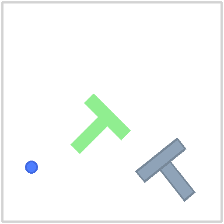
\includegraphics[width=2.55cm]{figures/split_assets/pusht.png}};
\node[heading] at (1.34,3.45) {Reacher};
\node[note,text=splitMuted] at (1.34,3.08) {density};
\node[inner sep=0pt] at (1.34,1.46)
  {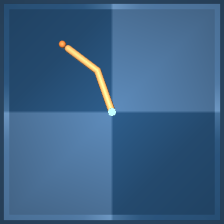
\includegraphics[width=2.55cm]{figures/split_assets/reacher.png}};

% One repeated observed state: only colors change between row headers.
\node[heading] at (4.11,6.98) {Appearance};
\node[note,text=splitMuted] at (4.11,6.59) {same state};
\foreach \row/\yy in {0/4.85,1/3.65,2/2.45,3/1.15}{
  \node[inner sep=0pt] at (4.15,\yy)
    {\includegraphics[width=1.08cm]{figures/split_assets/pusht_v\row.png}};
  \node[anchor=east] at (3.45,\yy) {$v_{\row}$};
}
\node[note,text=splitViolet] at (3.20,.80) {new};

% Same-input/different-response analogy. Lengths and rotations are non-quantitative.
\node[heading] at (9.30,6.98) {Dynamics};
\node[note,text=splitMuted] at (9.30,6.59) {same action; schematic responses};
\foreach \xx/\dx/\dy/\angle/\index in
  {6.35/.55/.03/10/0,8.35/.61/.13/-20/1,10.35/.55/.18/25/2,12.65/.63/.01/-10/3}{
  \begin{scope}[shift={(\xx,5.87)}]
    \fill[splitMuted] (-.61,-.06)--(-.30,-.06)--(-.30,.04)--(-.40,.04)
      --(-.40,.24)--(-.51,.24)--(-.51,.04)--(-.61,.04)--cycle;
    \fill[splitBlue] (-.80,-.10) circle (.059);
    \draw[actionarrow] (-.88,-.29)--(-.37,-.29);
    % Connector bounds are separated from both the initial and rotated response glyphs.
    \draw[responsearrow] (-.17,.04)--(.25,\dy+.03);
    \begin{scope}[shift={(\dx,\dy)},rotate=\angle]
      \draw[splitOrange,fill=splitOrange!18,line width=.65pt]
        (-.15,-.06)--(.15,-.06)--(.15,.04)--(.055,.04)
        --(.055,.24)--(-.055,.24)--(-.055,.04)--(-.15,.04)--cycle;
    \end{scope}
  \end{scope}
  \node at (\xx,5.35) {$p_{\index}$};
}
\node[note,text=splitViolet,anchor=west] at (12.93,5.35) {new};

% A quiet crossing map: positions carry the split, symbols carry membership.
\fill[splitPale,rounded corners=4pt] (5.42,1.88) rectangle (11.27,5.11);
\foreach \yy in {4.25,3.05}{\draw[white,line width=1pt] (5.42,\yy)--(11.27,\yy);}
\foreach \xx in {7.35,9.35}{\draw[white,line width=1pt] (\xx,1.88)--(\xx,5.11);}
\draw[splitViolet!65,densely dashed,line width=.75pt] (11.63,.62)--(11.63,6.02);
\draw[splitViolet!65,densely dashed,line width=.75pt] (3.57,1.80)--(13.65,1.80);
\foreach \xx/\yy in {6.35/4.85,8.35/4.85,10.35/4.85,6.35/3.65,10.35/3.65,6.35/2.45,8.35/2.45}{
  \pic at (\xx,\yy) {train};
}
\pic at (8.35,3.65) {dev};
\pic at (10.35,2.45) {heldout};
\foreach \xx/\yy in {12.65/4.85,6.35/1.15,12.65/1.15}{\pic at (\xx,\yy) {extra};}

% One legend; no repeated prose in cells. Blank intersections are untested.
\pic at (4.06,.20) {train};
\node[note,anchor=west] at (4.31,.20) {Train (7)};
\pic at (6.07,.20) {dev};
\node[note,anchor=west] at (6.36,.20) {Dev.};
\pic[scale=.70] at (7.68,.20) {heldout};
\node[note,anchor=west] at (7.96,.20) {Held-out pair};
\pic at (10.70,.20) {extra};
\node[note,anchor=west] at (11.02,.20) {Extrapolation};
\end{tikzpicture}%
\endgroup%
